% =========================================================================
% fig_hd3_triangulo_metropolitano_redundancia.tex
% Metropolitan N-1 strategic redundancy triangle: JSAURI — PALAMARA — SCN
% Exact to-scale geometry (0.14 cm/km): 70.5 / 22.1 / 50.0 km
% Dossier: TPWRS-SENI-142-2026 — data: one-line diagram + ARTEFACTO_B1 (sealed)
% =========================================================================
\documentclass[tikz,border=12pt]{standalone}
\usepackage[T1]{fontenc}
\usepackage[utf8]{inputenc}
\usepackage{amsmath}
\usepackage{booktabs}
\usetikzlibrary{arrows.meta,positioning,calc,decorations.markings}
\definecolor{seniNavy}{RGB}{26,54,93}
\definecolor{seniRed}{RGB}{155,44,44}
\definecolor{seniBlue}{RGB}{43,108,176}
\definecolor{seniGold}{RGB}{190,140,40}
\definecolor{seniGreen}{RGB}{39,103,73}
\tikzset{>={Stealth[length=2.5mm,width=1.8mm]},
         lbl/.style={font=\footnotesize,align=left},
         lblS/.style={font=\scriptsize,align=left}}
\begin{document}
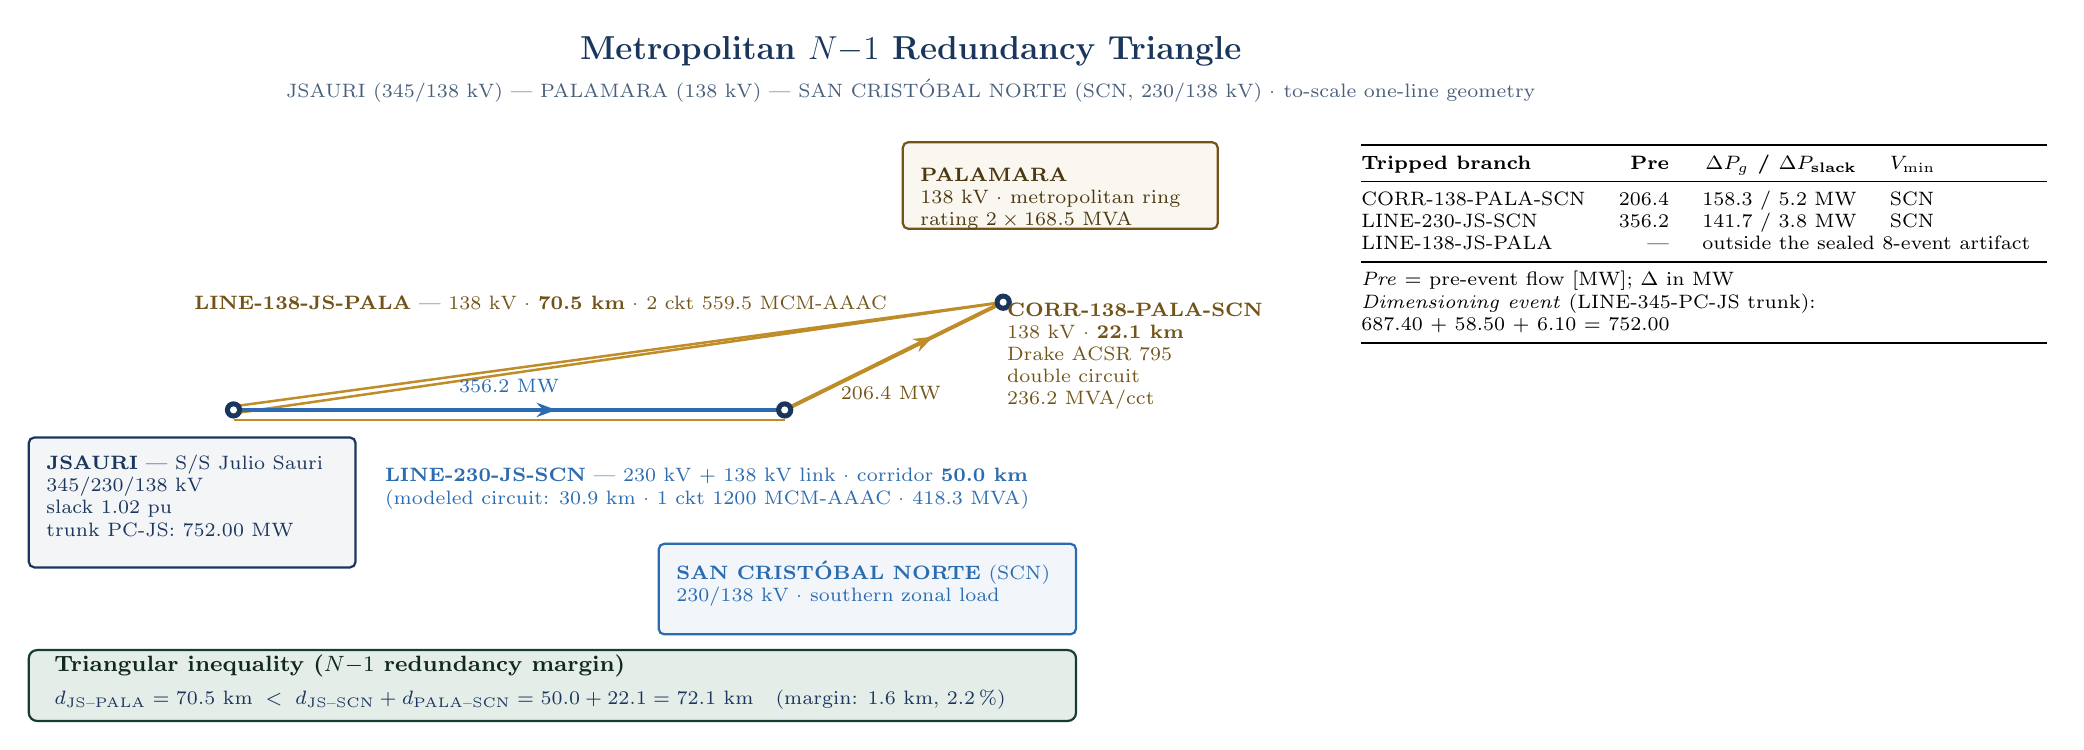
\begin{tikzpicture}[x=1cm,y=1cm]

% --------------------------------------------------------------- title
\node[lbl,font=\large\bfseries,seniNavy] at (8.6,4.55)
  {Metropolitan $N{-}1$ Redundancy Triangle};
\node[lblS,seniNavy!80] at (8.6,4.05)
  {JSAURI (345/138 kV) — PALAMARA (138 kV) — SAN CRIST\'OBAL NORTE (SCN, 230/138 kV) · to-scale one-line geometry};

% ------------------------------------------- vertices (0.14 cm = 1 km)
% JS=(0,0)  SCN=(50 km -> 7.0, 0)  PALA=(69.82 km -> 9.775, 9.77 km -> 1.368)
\coordinate (JS)   at (0,0);
\coordinate (SCN)  at (7.0,0);
\coordinate (PALA) at (9.775,1.368);

% side JS-PALA: 2 x 138 kV circuits
\foreach \dy in {-0.045,0.045}{
  \draw[seniGold,line width=0.9pt] (JS) -- ++(0,\dy) -- ([yshift=\dy]PALA);}
% side PALA-SCN: Drake double circuit
\foreach \dy in {-0.06,0.06}{
  \draw[seniGold,line width=1.3pt] ([yshift=\dy]SCN) -- ([yshift=\dy]PALA);}
% side JS-SCN: 230 kV + 138 kV link
\draw[seniBlue,line width=1.4pt] (JS) -- (SCN);
\draw[seniGold,line width=0.6pt] (0,-0.13) -- (7.0,-0.13);

% pre-event flow arrows (midpoint of each supplied side)
\draw[->,seniBlue,line width=1.4pt] (2.9,0) -- (4.1,0);
\node[lblS,seniBlue,anchor=south] at (3.5,0.1) {356.2~MW};
\draw[->,seniGold,line width=1.3pt] ($(SCN)!0.42!(PALA)$) -- ($(SCN)!0.68!(PALA)$);
\node[lblS,seniGold!60!black,anchor=north] at (8.35,0.42) {206.4~MW};

% vertices
\fill[seniNavy] (JS) circle (0.11);
\fill[white]    (JS) circle (0.045);
\fill[seniNavy] (SCN) circle (0.11);
\fill[white]    (SCN) circle (0.045);
\fill[seniNavy] (PALA) circle (0.11);
\fill[white]    (PALA) circle (0.045);

% substation boxes
\draw[seniNavy,thick,rounded corners=2pt,fill=seniNavy!5] (-2.6,-0.35) rectangle (1.55,-2.0);
\node[lblS,anchor=north west,seniNavy] at (-2.5,-0.45)
  {\textbf{JSAURI} — S/S Julio Sauri\\ 345/230/138 kV\\ slack 1.02 pu\\ trunk PC-JS: 752.00 MW};
\draw[seniGold!60!black,thick,rounded corners=2pt,fill=seniGold!7] (8.5,2.3) rectangle (12.5,3.4);
\node[lblS,anchor=north west,seniGold!40!black] at (8.6,3.2)
  {\textbf{PALAMARA}\\ 138 kV · metropolitan ring\\ rating $2\times168.5$~MVA};
\draw[seniBlue,thick,rounded corners=2pt,fill=seniBlue!6] (5.4,-1.7) rectangle (10.7,-2.85);
\node[lblS,anchor=north west,seniBlue] at (5.5,-1.8)
  {\textbf{SAN CRIST\'OBAL NORTE} (SCN)\\ 230/138 kV · southern zonal load};

% side labels
\node[lblS,seniGold!60!black,anchor=south] at (3.9,1.15)
  {\textbf{LINE-138-JS-PALA} — 138 kV · \textbf{70.5 km} · 2 ckt 559.5 MCM-AAAC};
\node[lblS,seniGold!60!black,anchor=west] at (9.7,0.68)
  {\textbf{CORR-138-PALA-SCN}\\ 138 kV · \textbf{22.1 km}\\ Drake ACSR 795\\ double circuit\\ 236.2 MVA/cct};
\node[lblS,seniBlue,anchor=north west,align=left] at (1.8,-0.62)
  {\textbf{LINE-230-JS-SCN} — 230 kV + 138 kV link · corridor \textbf{50.0 km}\\
   (modeled circuit: 30.9 km · 1 ckt 1200 MCM-AAAC · 418.3 MVA)};

% triangular inequality
\draw[seniGreen!60!black,thick,rounded corners=3pt,fill=seniGreen!12] (-2.6,-3.95) rectangle (10.7,-3.05);
\node[lbl,anchor=west,font=\footnotesize\bfseries,seniGreen!40!black] at (-2.4,-3.25)
  {Triangular inequality ($N{-}1$ redundancy margin)};
\node[lbl,anchor=west,font=\scriptsize,seniNavy] at (-2.4,-3.68)
  {$d_{\text{JS–PALA}} = 70.5~\text{km} \;<\; d_{\text{JS–SCN}} + d_{\text{PALA–SCN}} = 50.0 + 22.1 = 72.1~\text{km}$\quad (margin: 1.6 km, 2.2\,\%)};

% post-contingency table
\node[anchor=north west,font=\scriptsize,align=left] at (14.2,3.5)
  {\begin{tabular}{@{}lrrl@{}}
   \toprule
   \textbf{Tripped branch} & \textbf{Pre} & \textbf{$\Delta P_g$ / $\Delta P_{\text{slack}}$} & \textbf{$V_{\min}$} \\
   \midrule
   CORR-138-PALA-SCN & 206.4 & 158.3 / 5.2 MW & SCN \\
   LINE-230-JS-SCN   & 356.2 & 141.7 / 3.8 MW & SCN \\
   LINE-138-JS-PALA  & —     & \multicolumn{2}{l}{outside the sealed 8-event artifact} \\
   \midrule
   \multicolumn{4}{@{}l}{\emph{Pre} = pre-event flow [MW]; $\Delta$ in MW}\\
   \multicolumn{4}{@{}l}{\emph{Dimensioning event} (LINE-345-PC-JS trunk):}\\
   \multicolumn{4}{@{}l}{687.40 + 58.50 + 6.10 = 752.00}\\
   \bottomrule
   \end{tabular}};

\end{tikzpicture}
\end{document}
